\section{奇异同调中的切除}
\sourcepage{203}
本节验证奇异同调的切除公理。证明中使用的方法以后在其他场合也很有用。

关于单纯复形，我们曾证明：有限复形经过重心重分后，可以分割为任意小的单形。现在需要奇异链的一个类似结论。为精确表述，引入如下定义。

\entry{定义}{4.4.1}设 $\mathcal A$ 是空间 $X$ 的一些子集组成的族，它们的内部覆盖 $X$。若一个奇异单形的像完全包含于 $\mathcal A$ 的某个成员，则称它为\textbf{$\mathcal A$-小的}（$\mathcal A$-small）。

给定 $X$ 中的奇异链，我们将把它“分割”，使其中的所有单形均为 $\mathcal A$-小的。为此，自然要引入类似重心重分的运算。下面给出细节。

\entry{定义}{4.4.2}对拓扑空间 $X$，归纳定义同态 $\operatorname{sd}_X:S_p(X)\to S_p(X)$。若 $T:\Delta_0\to X$，令 $\operatorname{sd}_XT=T$。设已在小于 $p$ 的维数定义此同态。令 $i_p:\Delta_p\to\Delta_p$ 为恒等映射，$\widehat\Delta_p$ 为 $\Delta_p$ 的重心。用第 4.2 节的括号运算定义
\[
\operatorname{sd}_{\Delta_p}i_p=(-1)^p[\operatorname{sd}_{\Delta_p}(\partial i_p),\widehat\Delta_p].
\]
这一定义有意义，因为 $\Delta_p$ 关于其重心星形凸。对于任意奇异单形 $T:\Delta_p\to X$，令
\[
\operatorname{sd}_XT=T_\#(\operatorname{sd}_{\Delta_p}i_p).
\]
\sourcepage{204}
见图 4.4.1。称 $\operatorname{sd}_X$ 为奇异同调论中的\textbf{重心重分算子}（barycentric subdivision operator）。
\begin{center}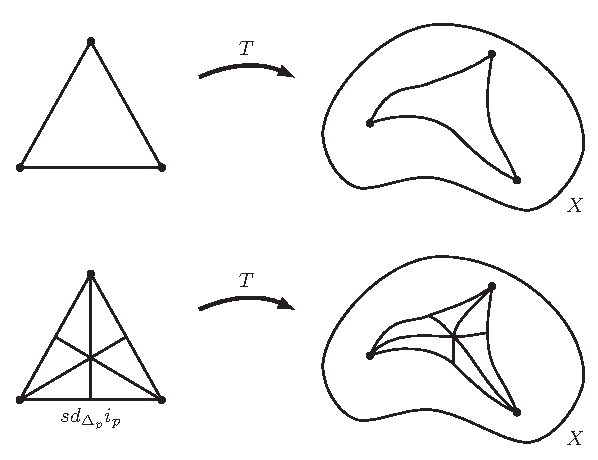
\includegraphics[width=.85\textwidth]{figures/4-4-1.pdf}\\图 4.4.1\end{center}

\entry{引理}{4.4.3}同态 $\operatorname{sd}_X$ 是保持增广的链映射，并具有自然性：对每个连续映射 $f:X\to Y$，有
\[
f_\#\circ\operatorname{sd}_X=\operatorname{sd}_Y\circ f_\#.
\]
\textbf{证明：}因为 $\operatorname{sd}_X$ 在零维为恒等同态，它保持增广，且在零维具有自然性。正维数中的自然性由直接计算得到：
\[
f_\#(\operatorname{sd}_XT)=f_\#T_\#(\operatorname{sd}_{\Delta_p}i_p)
=\operatorname{sd}_Y(f\circ T)=\operatorname{sd}_Y(f_\#T).
\]
以后通常省略下标，由上下文确定 $\operatorname{sd}$ 所指的空间。

\sourcepage{205}
为证明它是链映射，对 $p$ 归纳。零维中 $\operatorname{sd}\partial=\partial\operatorname{sd}$ 显然成立。设在小于 $p$ 的维数已成立。由引理 4.2.8，
\[
\partial\operatorname{sd}i_p=
\begin{cases}
(-1)^p[\partial\operatorname{sd}\partial i_p,\widehat\Delta_p]+\operatorname{sd}\partial i_p,&p>1,\\
-\epsilon(\operatorname{sd}\partial i_1)T_0+\operatorname{sd}\partial i_1,&p=1,
\end{cases}
\]
其中 $T_0$ 的像为 $\widehat\Delta_1$。若 $p>1$，归纳假设给出 $\partial\operatorname{sd}\partial i_p=\operatorname{sd}\partial\partial i_p=0$；若 $p=1$，由保持增广性，$\epsilon(\operatorname{sd}\partial i_1)=\epsilon(\partial i_1)=0$。因此两种情形都有 $\partial\operatorname{sd}i_p=\operatorname{sd}\partial i_p$。一般地，
\begin{align*}
\partial\operatorname{sd}T
&=\partial T_\#(\operatorname{sd}i_p) &&\text{（定义）}\\
&=T_\#(\partial\operatorname{sd}i_p)&&\text{（$T_\#$ 是链映射）}\\
&=T_\#(\operatorname{sd}\partial i_p)&&\text{（刚证明的公式）}\\
&=\operatorname{sd}T_\#(\partial i_p)&&\text{（自然性）}\\
&=\operatorname{sd}\partial(T_\#i_p)=\operatorname{sd}\partial T. &&\text{（$T_\#$ 是链映射）}
\end{align*}
\hfill$\square$

\entry{引理}{4.4.4}若 $T:\Delta_p\to\sigma$ 是到 $p$ 维单形 $\sigma$ 的线性同胚，则 $\operatorname{sd}T$ 的每一项都是从 $\Delta_p$ 到 $\sigma$ 的第一次重心重分中某个单形的线性同胚。

\textbf{证明：}$p=0$ 时显然。设结论在小于 $p$ 的维数成立。先考虑 $i_p:\Delta_p\to\Delta_p$。由定义，
\[
\operatorname{sd}i_p=(-1)^p[\operatorname{sd}\partial i_p,\widehat\Delta_p].
\]
\translatornote{原书在本证明此式中漏印了系数 $(-1)^p$；这不影响关于各项像集的论证。}链 $\partial i_p$ 的每一项都是从 $\Delta_{p-1}$ 到 $\Bd\Delta_p$ 中某个单形的线性同胚。由归纳假设，可写 $\operatorname{sd}\partial i_p=\sum\pm T_i$，其中 $T_i$ 是到 $\Bd\Delta_p$ 的第一次重心重分中某个单形 $\widehat s_1\cdots\widehat s_p$ 的线性同胚。于是 $[T_i,\widehat\Delta_p]$ 是到单形 $\widehat\Delta_p\widehat s_1\cdots\widehat s_p$ 的线性同胚，而该单形属于 $\Delta_p$ 的第一次重心重分。

对于一般的 $T$，由于线性同胚把各面的重心映为相应面的重心，它诱导 $\Delta_p$ 与 $\sigma$ 的第一次重心重分之间的线性同构。由 $\operatorname{sd}T=T_\#(\operatorname{sd}i_p)$，且线性同胚的复合仍为线性同胚，即得结论。\hfill$\square$

\sourcepage{206}
\entry{定理}{4.4.5}设 $\mathcal A$ 是 $X$ 的子集族，其成员的内部覆盖 $X$。给定 $T:\Delta_p\to X$，存在 $m$，使 $\operatorname{sd}^mT$ 的每一项都是 $\mathcal A$-小的。

\textbf{证明：}由上一引理迭代可知：若 $L:\Delta_p\to\sigma$ 为线性同胚，则 $\operatorname{sd}^mL$ 的每一项都是到 $\sigma$ 的第 $m$ 次重心重分中某个单形的线性同胚。

开集 $T^{-1}(\Int A)$（$A\in\mathcal A$）覆盖 $\Delta_p$。取这个开覆盖的 Lebesgue 数 $\lambda$（引理 2.4.1），并取 $m$ 足够大，使 $\Delta_p$ 的第 $m$ 次重心重分中的每个单形直径均小于 $\lambda$。于是 $\operatorname{sd}^mi_p$ 每一项的像集直径均小于 $\lambda$。因此 $\operatorname{sd}^mT=T_\#(\operatorname{sd}^mi_p)$ 中每一项的像都包含于某个 $A\in\mathcal A$。\hfill$\square$

既已说明怎样把奇异链分割为 $\mathcal A$-小的链，下面证明这些链足以生成 $X$ 的同调。先证明一个引理。

\entry{引理}{4.4.6}给定 $m$，对每个空间 $X$ 存在同态 $D_X:S_p(X)\to S_{p+1}(X)$，使对每个奇异单形 $T$ 有
\[
\partial D_XT+D_X\partial T=\operatorname{sd}^mT-T.\tag{*}
\]
而且 $D_X$ 是自然的：若 $f:X\to Y$，则 $f_\#D_X=D_Yf_\#$。

\textbf{证明：}零维中令 $D_XT=0$，则 (*) 及自然性显然成立。设 $p>0$，并设所有空间在小于 $p$ 的维数均已定义满足这些条件的 $D_X$。用与引理 4.3.6 类似的方法；下一节将把它表述为无环模型法。

先取 $X=\Delta_p$、$T=i_p$。令 $c_p=\operatorname{sd}^mi_p-i_p-D_{\Delta_p}(\partial i_p)$。用通常的计算及归纳假设可得 $\partial c_p=0$。因为 $\Delta_p$ 的奇异同调无环，可选取 $D_{\Delta_p}i_p\in S_{p+1}(\Delta_p)$，使其边缘为 $c_p$。于是此特殊情形满足 (*)。

对于任意 $T:\Delta_p\to X$，令 $D_XT=T_\#(D_{\Delta_p}i_p)$。计算得
\begin{align*}
\partial D_XT&=T_\#(\partial D_{\Delta_p}i_p)\\
&=T_\#(\operatorname{sd}^mi_p-i_p-D_{\Delta_p}\partial i_p)\\
&=\operatorname{sd}^mT_\#i_p-T_\#i_p-D_XT_\#\partial i_p\\
&=\operatorname{sd}^mT-T-D_X\partial T.
\end{align*}
倒数第二步使用了 $D_X$ 在 $(p-1)$ 维的自然性。$p$ 维的自然性则直接来自定义。\hfill$\square$

\sourcepage{207}
由 $\operatorname{sd}^m$ 与 $D_X$ 的自然性，若 $A\subset X$，它们分别把 $S_p(A)$ 映入 $S_p(A)$ 与 $S_{p+1}(A)$。故在相对链复形 $\mathcal S(X,A)$ 上，它们也分别诱导链映射与链同伦。

\entry{定义}{4.4.7}设 $\mathcal A$ 覆盖空间 $X$。以 $S_p^{\mathcal A}(X)$ 表示由 $\mathcal A$-小的奇异单形生成的 $S_p(X)$ 的子群，以 $\mathcal S^{\mathcal A}(X)$ 表示由这些链群组成的链复形。它是 $\mathcal S(X)$ 的子链复形：若 $T$ 的像包含于 $A\in\mathcal A$，则 $\partial T$ 每一项的像也包含于 $A$。

每个零维单形自动为 $\mathcal A$-小的，所以 $S_0^{\mathcal A}(X)=S_0(X)$，且 $\epsilon$ 给出其增广。\translatornote{原书此等式左端的下标印为 $p$；应为 $0$。}由上面的观察，$\operatorname{sd}^m$ 和 $D_X$ 都将 $\mathcal S^{\mathcal A}(X)$ 映入自身：若 $T$ 的像包含于 $A\in\mathcal A$，则它们作用后每一项的像仍包含于 $A$。

\entry{定理}{4.4.8}若 $\mathcal A$ 的成员的内部覆盖 $X$，则包含映射 $\mathcal S^{\mathcal A}(X)\to\mathcal S(X)$ 在普通及约化同调中均诱导同构。

\textbf{证明：}一个自然的想法是构造包含映射的链同伦逆 $\lambda:\mathcal S(X)\to\mathcal S^{\mathcal A}(X)$，但这并不容易。对任何特定的链，某个 $\operatorname{sd}^m$ 可以奏效；链变化时，所需的 $m$ 却可能越来越大。我们换一种方法。

考虑短正合列
\[
0\longrightarrow S_p^{\mathcal A}(X)\longrightarrow S_p(X)\longrightarrow S_p(X)/S_p^{\mathcal A}(X)\longrightarrow0.
\]
它给出普通或约化同调的长正合列。因此，只需证明商链复形 $\{S_p(X)/S_p^{\mathcal A}(X),\partial\}$ 在每一维的同调均为零。也就是说，若 $c_p\in S_p(X)$ 满足 $\partial c_p\in S_{p-1}^{\mathcal A}(X)$，只需找到 $d_{p+1}$，使 $c_p+\partial d_{p+1}\in S_p^{\mathcal A}(X)$。

链 $c_p$ 是有限个奇异单形的形式线性组合，由定理 4.4.5，可取统一的 $m$，使 $\operatorname{sd}^mc_p$ 中每个单形均为 $\mathcal A$-小的。取引理 4.4.6 中对应此 $m$ 的 $D_X$，则
\[
c_p+\partial D_Xc_p=\operatorname{sd}^mc_p-D_X\partial c_p.
\]
右端第一项按 $m$ 的选择属于 $S_p^{\mathcal A}(X)$，第二项因 $\partial c_p\in S_{p-1}^{\mathcal A}(X)$ 及前述保持性，也属于此群。取 $d_{p+1}=D_Xc_p$ 即可。\hfill$\square$

\sourcepage{208}
事实上，确实存在包含映射的链同伦逆 $\lambda:\mathcal S(X)\to\mathcal S^{\mathcal A}(X)$。[Vic73] 第 207 页给出了使用 $\operatorname{sd}^m$ 的具体公式。稍后我们还会从更一般的结果导出其存在性，见第 5.7 节习题。\translatornote{原书两处把链同伦逆的方向写成与包含映射相同；上文按其所需的逆向作了修正。}

\entry{推论}{4.4.9}设 $X$、$\mathcal A$ 同上，$B\subset X$。令 $S_p^{\mathcal A}(B)$ 由像包含于 $\mathcal A$ 某个成员的奇异单形 $T:\Delta_p\to B$ 生成，且令 $S_p^{\mathcal A}(X,B)=S_p^{\mathcal A}(X)/S_p^{\mathcal A}(B)$。则包含映射 $S_p^{\mathcal A}(X,B)\to S_p(X,B)$ 诱导同调同构。

\textbf{证明：}包含映射给出由两条短正合列
\begin{gather*}
0\longrightarrow\mathcal S^{\mathcal A}(B)\longrightarrow\mathcal S^{\mathcal A}(X)\longrightarrow\mathcal S^{\mathcal A}(X,B)\longrightarrow0,\\
0\longrightarrow\mathcal S(B)\longrightarrow\mathcal S(X)\longrightarrow\mathcal S(X,B)\longrightarrow0
\end{gather*}
导出的长正合列之间的同态。绝对同调上的同态由上一定理为同构，再由 Steenrod 五引理（引理 3.3.4），相对同调上的同态也为同构。\hfill$\square$

\entry{定理}{4.4.10（奇异同调的切除定理）}设 $A\subset X$。若 $U\subset X$ 满足 $\overline U\subset\Int A$，则包含映射
\[
j:(X\setminus U,A\setminus U)\to(X,A)
\]
在奇异同调中诱导同构。

\textbf{证明：}取 $\mathcal A=\{X\setminus U,A\}$。因为 $X\setminus\overline U\subset\Int(X\setminus U)$，且 $\overline U\subset\Int A$，这些集合的内部覆盖 $X$。考虑包含映射诱导的同态
\[
\frac{S_p(X\setminus U)}{S_p(A\setminus U)}\longrightarrow
\frac{S_p^{\mathcal A}(X)}{S_p^{\mathcal A}(A)}\longrightarrow
\frac{S_p(X)}{S_p(A)}.
\]
由上一推论，第二个同态诱导同调同构。下面证明第一个在链的层次上就已是同构。

\sourcepage{209}
包含映射诱导 $\varphi:S_p(X\setminus U)\to S_p^{\mathcal A}(X)/S_p^{\mathcal A}(A)$。若 $c_p\in S_p^{\mathcal A}(X)$，其每一项的像或包含于 $X\setminus U$，或包含于 $A$。形成模 $S_p^{\mathcal A}(A)$ 的陪集时，可删去后面这些项，所以 $\varphi$ 满射。而
\[
\ker\varphi=S_p(X\setminus U)\cap S_p^{\mathcal A}(A)
=S_p((X\setminus U)\cap A)=S_p(A\setminus U).
\]
故第一个同态为同构，证明完成。\hfill$\square$

这个定理比切除公理本身（第 3.5 节）略强：奇异同调论中不必假设 $U$ 是 $X$ 的开子集。作为应用，计算球和球面的奇异同调。

\entry{定理}{4.4.11}设 $n\ge0$。群 $H_i(B^n,S^{n-1})$ 在 $i=n$ 时为无限循环群，其余情形为零。群 $\widetilde H_i(S^n)$ 也在 $i=n$ 时为无限循环群，其余情形为零。反射映射
\[
\rho_1(x_1,x_2,\ldots,x_{n+1})=(-x_1,x_2,\ldots,x_{n+1})
\]
在 $\widetilde H_n(S^n)$ 上诱导的同态是乘以 $-1$。

\entry{注}{4.4.12}回忆定义 2.9.1，$n\ge1$ 时，这说明反射映射的度为 $-1$。

\textbf{定理的证明：}先设 $n=0$。空间 $B^0$ 为单点空间，$S^{-1}=\varnothing$，因为单位球面上的点必须有范数 $1$。由定理 4.3.3，$H_p(B^0,\varnothing)$ 在 $p=0$ 时为无限循环群，其余为零。

将定理 4.3.3 的证明推广到双点空间 $S^0=\{-1,+1\}$，可得 $p>0$ 时 $H_p(S^0)=0$，且 $H_0(S^0)=\Z\oplus\Z$，基为 $T_{-1}$、$T_{+1}$。所以 $\widetilde H_0(S^0)$ 为无限循环群，生成元为 $T_{+1}-T_{-1}$。映射 $\rho_1$ 交换两个点，故诱导同态为乘以 $-1$。

现作归纳。设定理在 $n-1$ 维成立，$n\ge1$。因 $B^n$ 可缩，$(B^n,S^{n-1})$ 的长正合列给出
\[
H_i(B^n,S^{n-1})\cong\widetilde H_{i-1}(S^{n-1}).
\]
所以左端在 $i=n$ 时为无限循环群，其余为零。

\sourcepage{210}
\begin{center}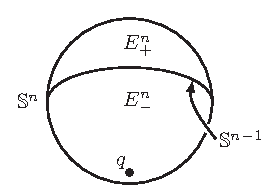
\includegraphics[width=.45\textwidth]{figures/4-4-2.pdf}\\图 4.4.2\end{center}
为计算 $\widetilde H_i(S^n)$，考虑同态图
\[
\begin{array}{ccc}
H_i(E^n_+,S^{n-1})&\xrightarrow{\partial_*}&\widetilde H_{i-1}(S^{n-1})\\
\downarrow\scriptstyle k_*&&\\
H_i(S^n\setminus\{q\},E^n_-\setminus\{q\})&&\\
\downarrow\scriptstyle j_*&&\\
H_i(S^n,E^n_-)&\xleftarrow{\ i_*\ }&\widetilde H_i(S^n),
\end{array}
\]
其中 $i,j,k$ 均为包含映射，$q=(0,\ldots,0,-1)$ 为南极。我们将证明四个同态 $i_*,j_*,k_*,\partial_*$ 都是同构，从而得到 $\widetilde H_i(S^n)\cong\widetilde H_{i-1}(S^{n-1})$。

回忆 $E^n_+$、$E^n_-$ 分别为上下半球，而 $S^{n-1}=E^n_+\cap E^n_-$ 是赤道。两个半球都是 $n$ 维球：$\R^{n+1}$ 到 $\R^n\times\{0\}$ 的投影把每个半球同胚地映到 $B^n$，也把 $E^n_-\setminus\{q\}$ 同胚地映到 $B^n\setminus\{0\}$。

特别地，$E^n_-$ 可缩，故 $(S^n,E^n_-)$ 的长正合列说明 $i_*$ 为同构。因 $q\in\Int E^n_-$，切除定理说明 $j_*$ 为同构。又因 $S^{n-1}$ 是 $E^n_-\setminus\{q\}$ 的形变收缩核，而 $E^n_+$ 是 $S^n\setminus\{q\}$ 的形变收缩核，$k_*$ 也是同构。〔空间偶 $(E^n_-\setminus\{q\},S^{n-1})$ 同胚于 $(B^n\setminus\{0\},S^{n-1})$，因而有到赤道的形变收缩 $F_t$；在 $E^n_+$ 上令每个 $F_t$ 为恒等映射，就将它延拓为 $S^n\setminus\{q\}$ 到 $E^n_+$ 的形变收缩。〕最后，$E^n_+$ 可缩，故 $\partial_*$ 为同构。归纳假设遂给出球面同调的结论。

反射 $\rho_1$ 将 $q$、上下半球及球面分别映入自身，故诱导上图到自身的同态。按归纳假设，它在 $\widetilde H_{n-1}(S^{n-1})$ 上为乘以 $-1$；由图中各同构及自然性，在 $\widetilde H_n(S^n)$ 上也如此。\hfill$\square$

\sourcepage{211}
注意上述证明中，真正直接计算的只有单点空间和双点空间的同调群。

\entry{推论}{4.4.13}若 $a:S^n\to S^n$ 是对径映射 $a(x)=-x$，则 $a_*$ 是乘以 $(-1)^{n+1}$。

\subsection*{习题}
\begin{enumerate}
\item 把引理 4.4.3、4.4.6 的自然性表述为 $\operatorname{sd}$、$D_X$ 是某些函子之间的自然变换。
\item 设 $X=\{(x,y):1<x^2+y^2<4\}\subset\R^2$ 为圆环，$\mathcal A$ 是平面内所有开圆盘组成的族。给出一个 $X$ 中 $\mathcal A$-小的奇异单形。
\item 对 $\R^3$ 中的单位球面 $X$，以及所有棱平行于坐标轴的开立方体组成的族 $\mathcal A$，重复习题 2。
\end{enumerate}
